% Journal-scale overview designed close to the manuscript text width.
% Only modest final scaling is needed, preserving readable labels.
\begingroup
\begin{tikzpicture}[
  font=\sffamily\scriptsize,
  >=Latex,
  main/.style={->, line width=0.75pt, draw=black!72},
  feature/.style={->, line width=0.75pt, draw=blue!67!black},
  guidance/.style={->, line width=0.75pt, dashed, draw=orange!82!black},
  section/.style={draw=black!17, rounded corners=2pt, fill=black!1},
  stage/.style={draw=blue!58!black, rounded corners=2pt, fill=blue!5,
    minimum width=17mm, minimum height=14mm, align=center, inner sep=1.5pt},
  merge/.style={draw=black!38, rounded corners=1pt, fill=black!4,
    minimum width=5mm, minimum height=7mm, align=center, inner sep=0.7pt},
  projection/.style={draw=teal!62!black, rounded corners=1.5pt, fill=teal!5,
    minimum width=17mm, minimum height=8.5mm, align=center, inner sep=1.2pt},
  decoder/.style={draw=violet!58!black, rounded corners=1.5pt, fill=violet!5,
    minimum height=9mm, align=center, inner sep=1.2pt},
  head/.style={draw=orange!76!black, rounded corners=1.5pt, fill=orange!8,
    minimum height=10mm, align=center, inner sep=1.2pt},
  tap/.style={draw=blue!70!black, fill=blue!10, minimum size=2.2mm, inner sep=0pt},
  label/.style={font=\sffamily\scriptsize, text=black!72}
]

% Section backgrounds keep the hierarchy clear without a decorative outer frame.
\node[section, minimum width=91mm, minimum height=31mm, anchor=south west] at (2.15,2.55) {};
\node[font=\sffamily\footnotesize\bfseries, anchor=west] at (2.38,5.35)
  {Four-stage encoder};
\node[section, minimum width=111mm, minimum height=24mm, anchor=south west,
  fill=violet!1, draw=violet!18] at (2.15,0.02) {};
\node[font=\sffamily\footnotesize\bfseries, anchor=east, text=violet!65!black,
  fill=white, inner sep=1pt]
  at (12.82,2.29) {SRF decoder};

% Input, stem, and encoder stages.
\node[draw=black!45, fill=white, inner sep=1pt] (input) at (0.48,4.12)
  {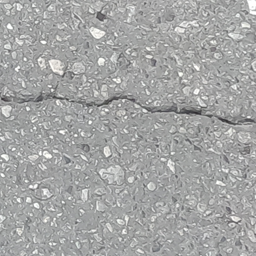
\includegraphics[width=8.5mm]{../dataset/CrackMap/test_img/GOPR0317 (5).png}};
\node[label, align=center, anchor=north] at ($(input.south)+(0,-0.10)$) {Input\\$512^2$};
\node[head, minimum width=8mm] (stem) at (1.52,4.12) {Stem\\$3{\to}16$};
\draw[main] (input) -- (stem);

\node[stage] (s1) at (3.20,4.12) {TransMixer\\\textbf{GAB}\\$16,\ 128^2$};
\node[merge] (m1) at (4.39,4.12) {PM\\$\downarrow2$};
\node[stage] (s2) at (5.58,4.12) {TransMixer\\\textbf{GAB}\\$32,\ 64^2$};
\node[merge] (m2) at (6.77,4.12) {PM\\$\downarrow2$};
\node[stage] (s3) at (7.96,4.12) {TransMixer\\\textbf{GAB}\\$64,\ 32^2$};
\node[merge] (m3) at (9.15,4.12) {PM\\$\downarrow2$};
\node[stage] (s4) at (10.34,4.12) {TransMixer\\\textbf{GAB}\\$128,\ 16^2$};
\draw[main] (stem) -- (s1);
\draw[main] (s1) -- (m1);
\draw[main] (m1) -- (s2);
\draw[main] (s2) -- (m2);
\draw[main] (m2) -- (s3);
\draw[main] (s3) -- (m3);
\draw[main] (m3) -- (s4);

% Multi-level feature taps and channel projections.
\node[tap] (f1) at (3.20,2.76) {};
\node[tap] (f2) at (5.58,2.76) {};
\node[tap] (f3) at (7.96,2.76) {};
\node[tap] (f4) at (10.34,2.76) {};
\node[label, anchor=east] at ($(f1.west)+(-0.05,0)$) {$F_1$};
\node[label, anchor=east] at ($(f2.west)+(-0.05,0)$) {$F_2$};
\node[label, anchor=east] at ($(f3.west)+(-0.05,0)$) {$F_3$};
\node[label, anchor=east] at ($(f4.west)+(-0.05,0)$) {$F_4$};
\draw[feature] (s1.south) -- (f1);
\draw[feature] (s2.south) -- (f2);
\draw[feature] (s3.south) -- (f3);
\draw[feature] (s4.south) -- (f4);

\node[projection] (p1) at (3.20,1.72) {$1{\times}1$ projection\\$16{\to}8$};
\node[projection] (p2) at (5.58,1.72) {$1{\times}1$ projection\\$32{\to}8$};
\node[projection] (p3) at (7.96,1.72) {$1{\times}1$ projection\\$64{\to}8$};
\node[projection] (p4) at (10.34,1.72) {$1{\times}1$ projection\\$128{\to}8$};
\draw[feature] (f1) -- (p1);
\draw[feature] (f2) -- (p2);
\draw[feature] (f3) -- (p3);
\draw[feature] (f4) -- (p4);

% SRF: F1 supplies spatial attention; F2--F4 are aligned and calibrated.
\node[decoder, minimum width=17mm] (up1) at (3.20,0.62) {$F_1$ upsample\\to $512^2$};
\node[decoder, minimum width=18mm] (att) at (5.48,0.62) {Spatial attention\\$A=\sigma(\phi(F_1))$};
\node[decoder, minimum width=27mm] (align) at (8.25,0.62)
  {Align $F_{2:4}$ to $128^2$\\calibrate by $A$, upsample};
\draw[feature] (p1.south) -- (up1.north);
\draw[guidance] (p1.south) -- ++(0,-0.18) -| (att.north);
\draw[feature] (p2.south) -- ++(0,-0.12) -| (align.north west);
\draw[feature] (p3.south) -- (align.north);
\draw[feature] (p4.south) -- ++(0,-0.12) -| (align.north east);
\draw[guidance] (att) -- (align);

\node[decoder, minimum width=12mm] (cat) at (11.10,1.18) {Concat\\$32$ ch};
\node[decoder, minimum width=13mm] (fuse) at (12.45,1.18) {Conv + GN\\$32{\to}8$};
\node[head, minimum width=11mm] (pred) at (13.78,1.18) {Prediction\\head};
\node[draw=black!45, fill=white, inner sep=1pt] (output) at (15.08,1.18)
  {\includegraphics[width=8.5mm]{../results/probability_maps/triple_stack_v4_crackmap/validate_v3_msa_ocv_gbc_seed42/GOPR0317 (5)_pre.png}};
\node[label, align=center, anchor=north] at ($(output.south)+(0,-0.10)$) {Probability\\map};
\draw[feature] (up1.east) -- ++(0.34,0) |- (cat.west);
\draw[feature] (align.east) -- ++(0.30,0) |- (cat.south);
\draw[main] (cat) -- (fuse);
\draw[main] (fuse) -- (pred);
\draw[main] (pred) -- (output);

% Compact legend.
\draw[main] (0.18,0.24) -- (0.76,0.24);
\node[label, anchor=west] at (0.82,0.24) {feature path};
\draw[guidance] (0.18,-0.02) -- (0.76,-0.02);
\node[label, anchor=west] at (0.82,-0.02) {$F_1$-guided calibration};

\end{tikzpicture}
\endgroup
